\subsection{ADC}
Tussen het filter en de digitale signaalverwerking zit een ADC blok, zoals te zien is in \cref{fig:ADCInSchema}. Dit blok converteert een analoge ingangsspanning naar een digitaal uitgangssignaal.

\begin{figure}[!htbp]
    \centering
    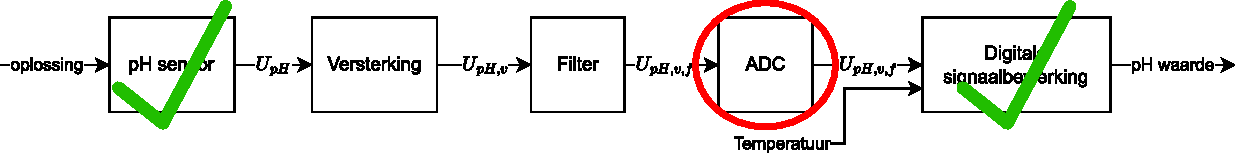
\includegraphics[width=0.95\textwidth]{signaalverwerking_ADC}
    \caption{Het onderdeel van \cref{fig:analogeBewerkingsFunctie} waar de spanningsreferentie zich in bevindt.}
    \label{fig:ADCInSchema}
\end{figure}

Het ADC blok, te zien in \cref{fig:ADCBlok}, heeft een gefilterde pH-afhankelijke spanning als ingang. De uitgang is een pH-afhankelijke digitale waarde.

\begin{figure}[!htbp]
    \centering
    \def\svgwidth{0.4\textwidth}
    \input{img/ADCBlok.pdf_tex}
    \caption{Het ADC blok.}
    \label{fig:ADCBlok}
\end{figure}

% min bits
Voor het omzetten van een analoog naar een digitaal signaal, heeft een ADC een zekere resolutie. Als deze resolutie niet hoog genoeg is, kan dit fouten introduceren. De resolutie is afhankelijk van het aantal bits dat de ADC heeft. Een andere oorzaak van fouten die bij een ADC kunnen optreden is de sample frequentie. Als deze niet hoog genoeg is zal dit ook een fout creëren.

\subsubsection{Aantal bits} \label{sec:ADC:numBits}
De resolutie van een ADC kan uitgerekend worden met \cref{eq:adcRes}, waarbij $n$ het aantal bits van de ADC is.
\begin{equation}\label{eq:adcRes}
    Q=\frac{1}{2^n-1}
\end{equation}

Met \cref{eq:meanSquareErrorADC} is de fout die ontstaat door de eindige resolutie van de ADC te berekenen \cite{MJHcalcADC}. Wanneer er uit specificaties een maximale $\overline{e_{eff}^2}$ kan worden gehaald kan met \cref{eq:calcNeededQ}, kan de minimale benodigde resolutie worden berekend.
\begin{equation}\label{eq:meanSquareErrorADC}
    \overline{e_{eff}^2}=\frac{Q^2}{12}
\end{equation}
\begin{equation}\label{eq:calcNeededQ}
    Q=\sqrt{12\cdot\overline{e_{eff}^2}}
\end{equation}

% $\overline{e_{eff}^2}$ mag niet groter dan de helft van het ingangsruis vermogen zijn (noise figure van 1.5dB).
Voor dit ontwerp is er een noise figure gegeven en is de SNR voor het kleinste signaal bekend. Ook is het kleinste ingangssignaal bekend. Door gebruik te maken van \cref{eq:calcSpecifiedRmsError}, is het mogelijk om uit te rekenen hoe groot de fout ten gevolge van de eindige resolutie van de ADC mag zijn.
\begin{equation}\label{eq:calcSpecifiedRmsError}
    \overline{e_{eff}^2}=\left(10^{\frac{NF}{10}}-1\right)\left(\frac{S_{rms}}{10^{\frac{SNR+NF}{20}}}\right)^2
\end{equation}

Door gebruik te maken van \cref{eq:adcRes,eq:meanSquareErrorADC,eq:calcSpecifiedRmsError}, kan het minimum aantal bits van de benodigde ADC berekend worden met \cref{eq:calcMinNumberADCbits}.
\begin{equation}\label{eq:calcMinNumberADCbits}
    n=\left\lceil\log_2\left(\frac{1}{Q}+1\right)\right\rceil
    \tagaddtext{[bits]}
\end{equation}

\subsubsection{Sample frequentie}\label{sec:ADC:sampleFreq}
% min sample rate
De hoogst nuttige sample frequentie voor een gegeven ADC is afhankelijk van het aantal bits van de ADC en de hoogste te meten signaal frequentie. Op deze sample frequentie zullen er ook geen fouten meer voorkomen ten gevolge van de sample frequentie \cite{MJHcalcADC}. De formule om deze sample frequentie mee te berekenen is gegeven door \cref{eq:ADCmaxFs}.
\begin{equation}\label{eq:ADCmaxFs}
    f_{s,max}=2^n\pi f_h
    \tagaddtext{[\si{\hertz}]}
\end{equation}
In veel gevallen is de hoogste sample rate niet van interesse omdat die zo hoog ligt dat het een puur theoretisch getal is. Om een minimale sample frequentie te berekenen moet er eerst een toe te stane fout bepaald worden. Deze fout kan door middel van een noise figure gespecificeerd worden. Met een bekende noise figure kan er door middel van \cref{eq:ADCmaxSampleError} een factor $E$ berekend worden. Deze factor kan worden gebruikt in \cref{eq:ADCminFs} om de minimale sample frequentie uit te rekenen.
\begin{equation}\label{eq:ADCmaxSampleError}
    E=10^{\frac{-NF}{10}}
\end{equation}
\begin{equation}\label{eq:ADCminFs}
    f_{s,min}=\frac{\pi f_h}{E}
    \tagaddtext{[\si{\hertz}]}
\end{equation}